\chapter{Implementation} \label{implementation}
This chapter describes how the approach we proposed in Chapter \ref{approach} is applied by using the Python API offered by CARLA. Moreover, we reveal the software implementation of the processes behind each of the three stages in our simulation pipeline.  

\section{Setup of Virtual Environment}
The simulation pipeline consists of three main stages - Data Generation for the experiments, Simulation of possible real-world scenarios and Evaluation of the results, as it was explained in the previous chapter. In the course of our first stage, we connect the client to the simulator's server, which represents the digital world for our research. The 3D simulator provides two options for a communication between client and server\footnote{\url{https://carla.readthedocs.io/en/latest/adv_synchrony_timestep/}, visited on 02/12/2022}:
\begin{itemize}
    \item \textbf{synchronous mode} - in this mode the client must notify via tick\footnote{Signal in CARLA for the server} when all the commands are prepared that the server is obliged to execute. This is the mode which is relevant for simulations where synchrony between, i.e., sensors and world is crucial. 
    \item \textbf{asynchronous mode} - this is the default mode, where the server runs the simulation as fast as possible and does not have to wait for a signal from the client, which ensures that everything is ready for the next step 
\end{itemize}

For this work the synchronous mode is set, because we require an environment, where we know location and rotation of world objects, receive accurate data from the camera and maintain a consistent connection to the server. When we enable the synchronous mode, we create a synchronous instance of the Traffic Manager, which handles any group of vehicles in the simulated world. For our experiments, we rely on the virtual city map "Town10HD\_Opt" and define good weather conditions, which do not affect the performance of the camera because we need optimal results in ideal conditions. Additionally, we remove the layer with parked vehicles, because otherwise they will be detected by the sensor and increase the number of pixels containing vehicles which are not important for the simulation.

\subsection{Sensor placement}
Having all synchrony-related settings adjusted, we then instantiate a new object of type Sensor from CARLA's blueprint library\footnote{\url{https://carla.readthedocs.io/en/latest/bp_library/}, visited on 03/12/2022}. This is a subtype of actor which can measure and stream data. For this thesis the sensor is instance segmentation camera which has the main parameters of each camera sensor: field of view, width and height of generated image. What is more, a sensor is responsible for perceiving data either whenever a new event is registered or on each tick-signal received from the client. This sensor in particular has a task to render all elements contained in the field of view with a specific colour according to their semantic tags (vehicle, building, traffic light, etc.) and a unique object ID assigned by the Unreal Engine at the moment of instantiation. 

With regard to the spawning of sensor, in CARLA one can attach it to a vehicle and thus to visualise an on-board point of view. However, the goal of this thesis is to find an optimal position in the infrastructure, therefore we spawn our traffic monitoring tool as displayed in Figure \ref{fig:camera_positions} on particular locations. Again, there is no algorithm for locations generation, they are completely random and aim to compare three points in each border of the region of interest, which makes eight in total. In order to receive data, which is then forwarded along the pipeline for examination, sensors have an integrated listening method. In short, there we provide as an argument a function that inserts every new image in a queue, which then can be accessed during the evaluation part. At the end, we define height, rotation and tilt angle of the camera so that it points to the intersection and have an unobstructed view. More information about what values for the camera's attributes are set for the experiments is described in chapter \ref{evaluation}.

\subsection{Waypoints generation}
The last step from the first stage is generation of waypoints suitable for our experiments, where pairs of vehicles are going to be placed to recreate real-world situations and estimate occlusion percentage, because it prevents the camera from a correct perception of the surrounding environment. CARLA supports methods\footnote{\url{https://carla.readthedocs.io/en/latest/core_map/}, visited on 03/12/2022}, which allow a user to select a landmark on the map and spawn an object there. In order to extract these points from the simulator, we have to specify which area is of interest. As we previously mentioned, we do not consider cases where a vehicle is spawned on impermissible places like pavements or green spaces. Therefore, the task of this work requires only valid road lanes as spawn location. Moreover, the simulated world offers the opportunity to choose from points which belong to possible driving routes and the process is the following one:
\begin{enumerate}
    \item The user gives a location as input and the simulator returns the nearest waypoint to it that lies on the premises of our region of interest, which in our case is an intersection of four roads.
    \item Knowing this waypoint, one can request from the simulator to return the junction which contains it.
    \item The returned junction comes with a list of various waypoints, therefore it should be specified in a method for extraction that we only need positions on driving lanes.
    \item In the previous step, we receive a list of pairs of points, which mark the beginning and the end of a lane. With a for-loop we iterate through all pairs and use a method from the simulator that returns a list of waypoints in the direction of the line a specified distance apart from each other. The new list contains all points from the current waypoint to the end of its lane.
\end{enumerate}
It is beneficial for the needs of our experiments to be able to define what distance should exist between the spawn positions. To illustrate an exemplary situation we use Figure \ref{fig:distance_waypoints}, where the distance between each point in a single lane is set to five meters. When the preparation of vehicle spawn locations is done, the simulation starts and the process is explained in the following section.

\begin{figure} [h!]
    \centering
    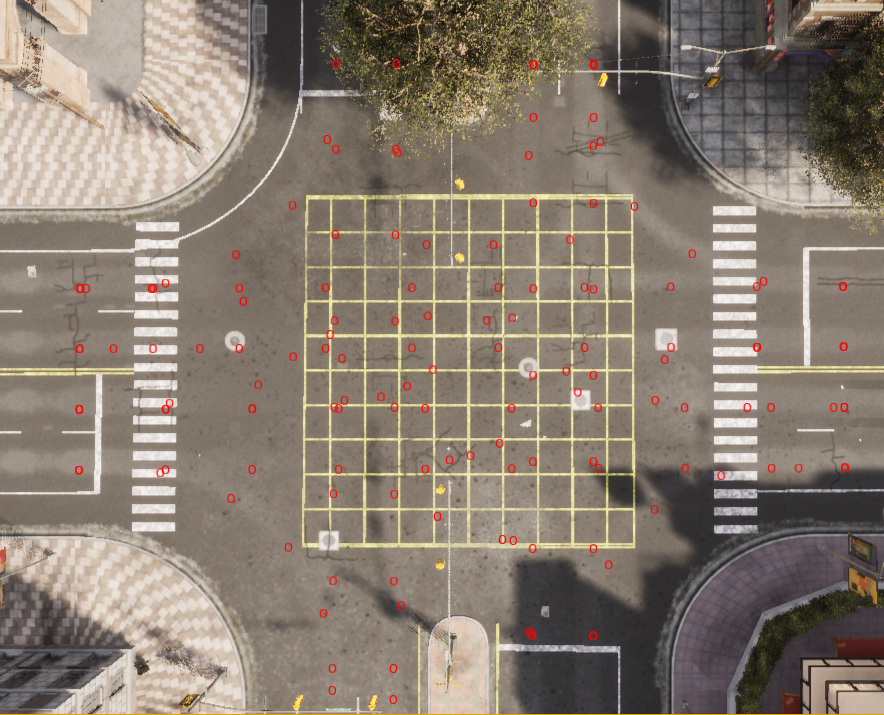
\includegraphics[width=0.75\textwidth]{images/waypoints_target.png}
    \caption[Vehicle waypoints with specified distance]{This image serves as an example of spawn points where we could place vehicles when the distance between them in each lane is 5 meters.}
    \label{fig:distance_waypoints}
\end{figure}

\section{Simulation of Valid Scenarios}
For the purpose of suggesting an optimal position for a camera sensor in the infrastructure that could enhance autonomous vehicles, improve communication between them and facilitate mobility per se, we have to reproduce real-world scenarios and observe how the sensor perform. The focus of this work is the occlusion, which occurs in everyday traffic when larger vehicles intercept a sensor's field of view, therefore we apply our own approach based on the Occlusion Degree Model proposed by Du et al. in \cite{occlusion_degree_model}. In subsection \ref{sec:sim_stage} we give a detailed explanation of how our experiments are designed, whereas here the technical means used by this stage are addressed.

\begin{figure} [h!]
    \centering
    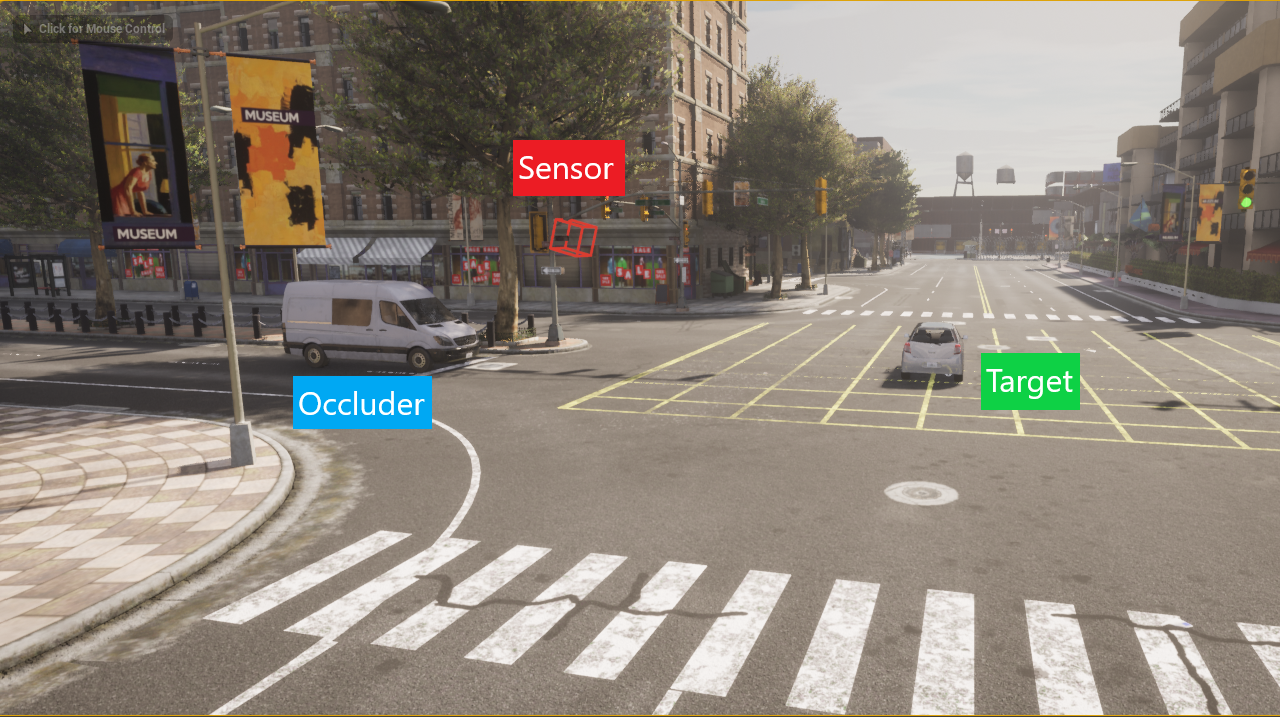
\includegraphics[width=0.85\textwidth]{images/behind_sensor.png}
    \caption[Vehicle spawned behind the camera]{We can see on this image a situation where the occluder is spawned out of the sensor's field of view, which makes it invisible for the sensor and is excluded from the experiment.}
    \label{fig:behind_sensor}
\end{figure}

\subsection{Spawning vehicles and their roles}
To start with, in each simulation we have two actor objects from type Carla.Vehicle, which can be chosen from the blueprint library\footnote{\url{https://carla.readthedocs.io/en/latest/bp_library/\#vehicle}, visited on 03/12/2022}. In this library a user can select whichever vehicle he needs for his purposes. In addition, vehicles are varying from motorcycles through small cars to large trucks. Again, our implementation inserts two vehicles in the virtual environment, which take the roles 'occluder' and 'target' depending on the vehicle's size. This means that if we put the label occluder to a vehicle 2x3m-sized vehicle and as a target vehicle we have a 4x8m-sized truck, it is certain that such scenario will be useless for experimental purposes, because in 95\% of the cases a normal object recognition algorithm would not have troubles in detecting it. For this reason, we suggest that always the occluder is larger than the target vehicle, which will guarantee more reliability of the results if this approach is to be adopted by further studies.

At the beginning, we generate a list of waypoints for both vehicles with a specified distance between them. Vehicles can only be spawned at the exact location of a waypoint and in the direction of the driving lane under them, which means that it is possible to spawn our actor on the same place multiple times but with different rotation. One important functionality of these waypoints is that the vehicle is always placed parallel to the ground and could not be hovering at an angle from thirty degrees, for example. Furthermore, this guarantees flexibility when simulating scenarios, because it is not necessary to always use a flat surface for the vehicles. 

Before placing the target on the first received waypoint, it is checked if the vehicle's centre is displayed on the image plane. The process is explained in subsection \ref{camera_model} and consists of several steps:
\begin{enumerate}
    \item World to camera matrix (W2C) generation - CARLA provides a method which returns the inverse matrix of the sensor as an array.
    \item Camera's intrinsic matrix $A$ generation - it contains the parameters of the sensor like coordinates of the principal point $u_0$ and $v_0$, skew index $\gamma=0$ (no distortion) and scale factors $\alpha$ and $\beta$ which have as a value the result of the focal length divided by the pixel size.
    \item 2D Projection of a 3D world point - we take the coordinates of the world point in an array, multiply it with the W2C matrix and change from Unreal Engine's coordinate system to a standard one $(x, y ,z) \rightarrow (y, -z, x)$. Afterwards, we multiply with the new array with the intrinsic matrix $A$ and both $x$ and $y$ are normalized by the third value in the array.
    \item If the final coordinates are negative or exceeds either the image's width or height then the vehicle is not spawned as it is practically invisible to the camera, and no occlusion could happen.
\end{enumerate}

When this check returns a positive output, the target vehicle is spawned in a height of 2 cm, as this is the minimum if we want the spawn to be successful, and then falls for some frames until it lands on the ground. We wait 20 frames until the physics are stabilised and the vehicle's z-coordinate remains constant. Then, we try to spawn the occluder vehicle on a location which is different from the target's one, because they cannot be spawned at the exact same point. We first check if the spawn point will cause an occlusion by:
\begin{enumerate}
    \item Measuring the diagonal of the occluder vehicle and taking only such positions where the distance between target and occluder spawn point is not longer than the diagonal. This guarantees mainly situations with occlusion, because we exclude positions where the occluder is far from the target and does not cover it. Furthermore, average truck's size is 3-4 meters, therefore it won't obstruct the sensor's view if it stays under it.
    \item Checking if the distance between sensor and occluder is longer than the one between sensor and target, which prevents the camera from considering spawn points behind the target vehicle.
\end{enumerate}
The above described constraints optimise simulations and reduce execution time significantly, because we consider mainly occlusion-prone points. Afterwards, it is checked again whether the occluder is visible for the camera, i.e. in Figure \ref{fig:behind_sensor} the Mercedes Sprinter is behind the sensor and would cause no occlusion, therefore it won't be considered in the experiment, but if that is not the case, the occluder successfully gets placed on the virtual intersection. During each iteration the camera records the situation on the road and streams data for evaluation of the occlusion, which is explained in the next subsection. Then the occluder is destroyed and simulation continues while the list with spawn points is not empty.

\begin{figure} [h!]
  \centering
  \subfloat[Vehicle at the moment of spawn]{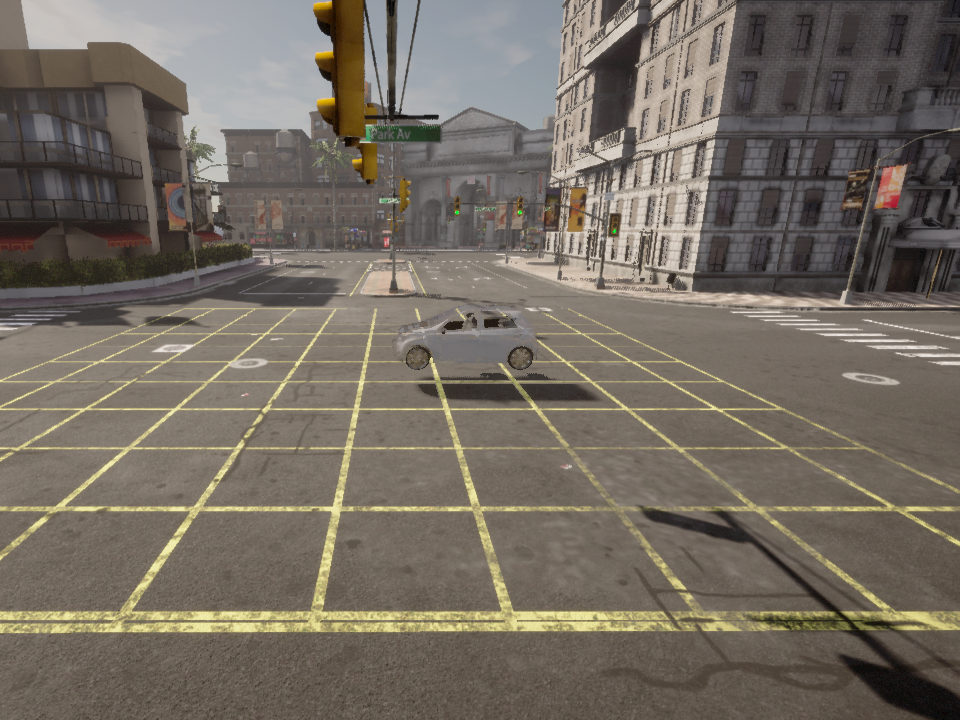
\includegraphics[width=0.5\textwidth]{images/spawn_air.jpg}}
  \hfill
  \subfloat[Vehicle on the ground]{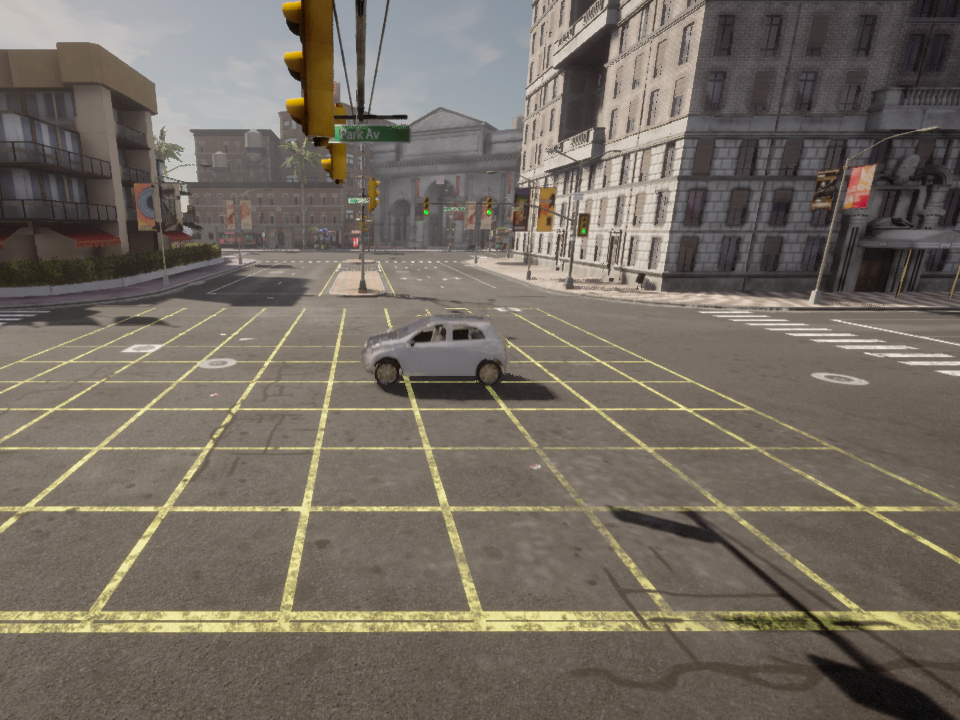
\includegraphics[width=0.5\textwidth]{images/spawn_ground.jpg}}
  \caption[Spawning a vehicle]{Both picture illustrate the described CARLA physics when a vehicle is spawned, it hovers first in the air and lands after some time on the ground.} \label{fig:spawn_vehicle}
\end{figure}

 \subsection{Camera output and occlusion calculation} \label{subsec:calc_occl}
 In this work the instance segmentation camera is used as a reliable sensor that provides only ground-truth data. An important advantage of this type of camera is that it can perform better than an object recognition method. However, it is still under development by the CARLA creators and has one drawback that after we spawn the target vehicle, we have to wait several ticks until it's displayed on the image plane. This happens because, as mentioned in the previous subsection, in the simulator a vehicle is always spawned in the air, therefore it needs some time to land on the ground and the world's physics to be stabilised as shown in Figure \ref{fig:spawn_vehicle}. Nevertheless, this issue does not cause any delays for the simulation.
 
 To calculate the occlusion, we need an image of the target vehicle alone and an image where both vehicles are available in the world. Therefore, the first image is taken after the target vehicle is spawned and when it already stays stationary on the ground. Subsequently, we try to spawn the occluder and take the image with both vehicles available in the simulator if it was successful. In the performed experiments, we do not wait for the occluders to be fully stationary, but only to be visible on the image plane, because this will increase execution time. This means, that the occlusion measured is no more than one percent higher than the real one. Again, result's accuracy is not heavily affected by this issue. For the calculation we use the following help methods:
 \begin{itemize}
     \item \textbf{Conversion of raw image data to a 2D array} - the data that is output by a camera is in a raw format, which should be transformed into a 2D array so that we could iterate through all pixels. This method extracts the blue, green and red values for each pixel and puts them in the exact row and column as the location of the pixels on the image plane. Blue and green channels define the object's unique ID, and the red one assigns it to a class according to its type.
     \item \textbf{Calculation of pixels containing a specific label} - in CARLA each item has a tag which defines the type of the object, e.g., whether it is a vehicle a building or something else. This method calculates how many pixels contain a given object type using the information from the red channel. 
 \end{itemize}

With the first help method we are able to generate arrays which we can iterate through, while the second one tells us how many pixels represent the target vehicle in an image, when the occluder is absent. We then iterate through the 2D array and consider only rows whose pixels contain objects from type vehicle. Inside each row we inspect again only columns containing a vehicle and calculate the ID of a vehicle using the blue and green value of a pixel. An important point to be made is that Unreal Engine gives an ID to each object spawned in the 3D world, which is not always the result of the expression \ref{eq:instance}, where B represents the blue value and G the green one.
When the ID crosses the hexadecimal value of $0\times10000$ which comprises 65536 in a decimal number system, we have to subtract this value from the object's ID so many times as it is contained in it, which is shown in the equation \ref{eq:new_id}.

\begin{equation}B + G * 256\label{eq:instance}\end{equation}

\begin{equation}\textrm{new\_ID} \: = \textrm{ID} - \lfloor \textrm{ID} / 65535 \rfloor * 65536\label{eq:new_id}\end{equation}

After we are done with the described calculations, we check if the occluder's ID equals the converted blue and green channels' values and increment the number of target's visible pixels. If we have reached a situation where the visible numbers are equal to all pixels from the first image, meaning the vehicle is not occluded, we break the loop and return the occlusion, which comprises the result of equation \ref{eq:occlusion}. In Figure \ref{fig:occlusion_calc} an example of two pictures used for estimation of the occlusion are provided, where the occlusion on the second one is 75\% and at this point exists a higher chance that the target vehicle is not detectable. Apart from the occlusion, the location of the target vehicle is also included in a text document after each iteration. 
% At the end of the simulation, we also add the number of times a vehicle was not visible on the camera and therefore not spawned to the document, which is crucial for the evaluation stage.  

\begin{equation}
    \frac{\textrm{target\_max\_pixels} - \textrm{target\_visible\_pixels}}{\textrm{target\_max\_pixels}} * 100 \label{eq:occlusion}
\end{equation}

\begin{figure} [h!]
  \centering
  \subfloat[Single target vehicle]{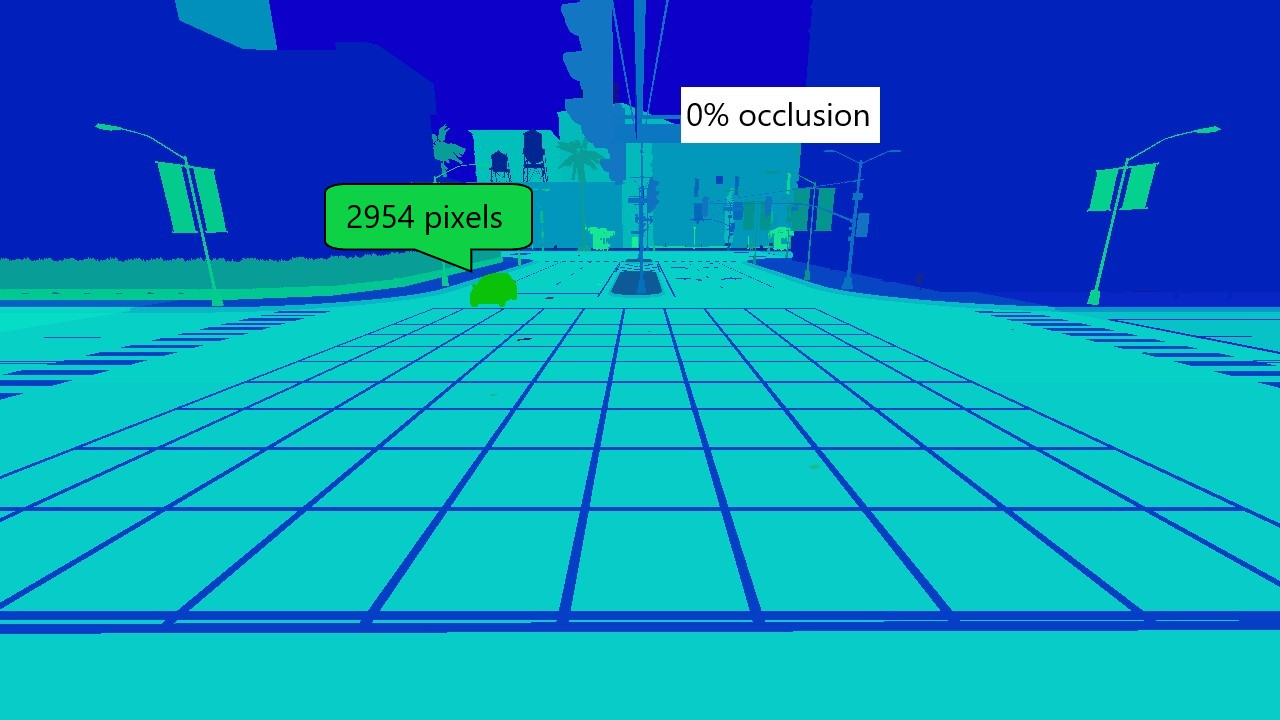
\includegraphics[width=0.5\textwidth]{images/before_occlusion.jpg}}
  \hfill
  \subfloat[Both occluder and target vehicles]{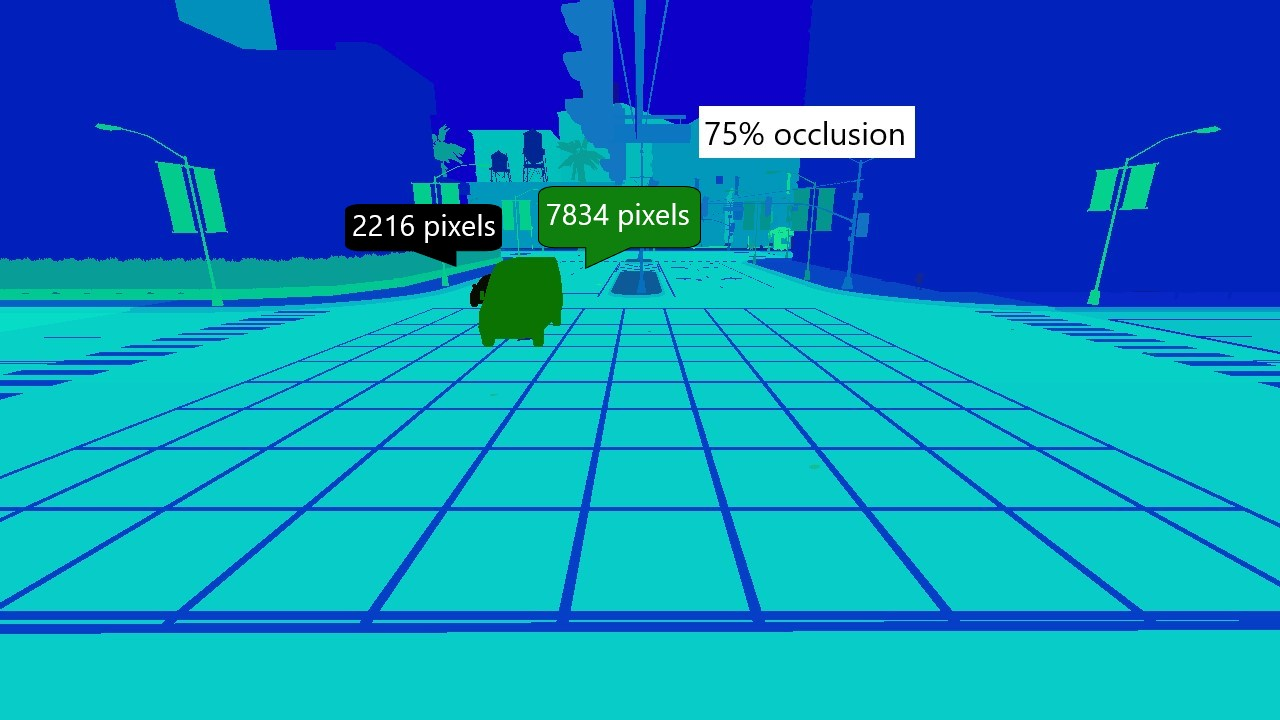
\includegraphics[width=0.5\textwidth]{images/after_occlusion.jpg}}
  \caption[Calculation of an occlusion]{The two images represent how vehicles are seen through the instance segmentation camera. On the right picture there is an occlusion of 75\%, visible pixels of each vehicle are shown in bubbles above them.} \label{fig:occlusion_calc}
\end{figure}
 
 \section{Evaluation of Results}
 In the final step of our simulation pipeline, we scrutinise our results to get an impression of which positions offer a more optimal sensor's performance. Due to the fact that our results are saved in a text file, we need some way of data visualisation, therefore heatmaps are chosen as the most suitable technique for displaying traffic data, i.e., in the studies \cite{heatmap_first, heatmap_second} also rely on heatmaps for their results. We mentioned previously that each row in the text file contains X and Y coordinates of a target's spawn location, as well as the occlusion degree. In order to display the results correctly on the heatmap, we first divide our region of interest - the intersection - into equal-sized $M \times N$ blocks where $M,N \in \mathbb{N}_{>0}$, so that we get a set of blocks denoted by $S$. Furthermore, the coordinates of a location are assigned to a block $B_{x,y} \in S$, which should represent the intersection's area on the heatmap. With regard to the heatmap's dimensions, they are defined by the absolute value of the difference between the minimum and maximum value of each coordinate, so that it contains all available spawn points from the ROI:
 \begin{equation}
     |x_{max} - x_{min}| + 1 = M
 \end{equation}
 \begin{equation}
     |y_{max} - y_{min}| + 1 = N
 \end{equation}
 
 Heatmaps require a 2D array, which they could read the information from. Additionally, dimensions of arrays cannot be negative values. In Unreal Engine's 3D world coordinates sometimes contain a negative value, which is problematic for the previous statement, and therefore we avoid this issue by converting each value accurately to a non-negative one using the following technique:
 \begin{enumerate}
     \item Find the minimal value $X_{min}$ among the X-coordinates in the list and round it, because we need non-decimal values for a heatmap's coordinates. In our case all x-coordinates have negative values.
     \item Take its absolute value $|X_{min}|$, iterate through each X-value and increment it with the absolute value. This step sets the lowest X-coordinate to be a starting point of the heatmap array. For example, if $X_{min} = -50$, each value will be then incremented by $50$.  
     \item Repeat steps 1 and 2 for each Y-coordinate value.
 \end{enumerate}
 In case the min-coordinates are positive numbers, we take their value with a minus sign in front of it and add it to each X and Y value respectively, so that the heatmap begins at $(0,0)$. For example, if $X_{min} = 5$, each X-coordinate will be decreased by $5$.
 
\begin{figure} [h!]
    \centering
    \includesvg[width=0.85\textwidth]{images/6m_target_heatmap.svg}
    \caption[Heatmap target full occlusion]{This image illustrates an example of how a heatmap would look like when the distance between waypoints is 6 m and the occlusion is 100\% on each location.}
    \label{fig:heatmap_target}
\end{figure}
 
\subsection{Occlusion degree and metrics} \label{subsec:metrics}
Our main criterion for an efficient position of a camera is when a low occlusion degree is estimated in the examined positions. During the simulation of occlusion-prone situations for our pair of vehicles, we can receive multiple values for a single target location, therefore we take the highest occlusion value for each point when generating a heatmap. 
% As a comparison, we also provide a heatmap that contains the average occlusion from all values found in the text file for each single spawn point (see equation \ref{eq:avg_occl}). However, we do not consider the lack of occlusion when calculating the average occlusion.  

% \begin{equation}
%     \textrm{avg\_occlusion\_degree} = \textrm{sum\_of\_occlusion\_for\_current\_location} / \textrm{location\_occurences}\label{eq:avg_occl}
% \end{equation}

When we calculate the occlusion degree, we set the value in a 2D array on the position $\textrm{array}[y,x]$. The reason for changing the order of coordinates is that the Python data visualisation library Seaborn\footnote{\url{https://seaborn.pydata.org/}, visited on 04/12/2022} we use is based on Matplotlib\footnote{\url{https://matplotlib.org/}, visited on 04/12/2022}, which reads first the y-dimension of the array and then the x-dimension, e.g., if we have an occlusion 40\% for the location $(x=12,y=5)$, then we have to request the element on position $(5,12)$ from the array. When everything is set correctly in the array, we plot the result using the "YlGnBu" (yellow-green-blue) colour palette, which displays the low values using light yellow colour and dark blue colour for the higher ones. We can see in Figure \ref{fig:heatmap_target} how the results for each target location at 6 m distance from each other are presented when there is a full occlusion everywhere. 

Apart from the occlusion, we also have two metrics, which are responsible for a better estimation of the experiment data. Our goal is to find a camera position, which minimises the score of the two metrics. In a real-life scenario it is impossible for a monocular camera to detect each vehicle in its field of view, when another vehicle has occluded it, which increases the chance for accidents to happen, e.g., if a truck stays in front of a small car, then the camera won't be able to detect the car and will act if it does not exists. For this reason, we want to have the minimum number of undetected vehicles due to a high occlusion degree (see M1). In addition, our motivation for the second strategy is to be able to avoid as many occlusions perceived by the camera as possible, and if this cannot happen to only have a few locations in the region of interest where this phenomenon occurs (see M2). We list our metrics below.

M1 - Undetected Vehicles due to a High Occlusion. It calculates the ratio of all times the occlusion exceeded a previously specified threshold $T$ to all times an occlusion greater than $0\%$ was detected. For a camera to be efficient, it is necessary that we get a low value for the tested position.
\begin{equation}
   M1 = \frac{\sum\textrm{occlusion}_{T}}{\sum\textrm{occlusion}_{>0}}
\end{equation}

M2 - Occlusion Occurrences Ratio. In order to calculate this metric, we collect information from the text file for each target position observed. We divide the times when an occlusion has occurred to all the times when we spawned a pair of vehicles and performed a calculation. To clarify, we strive again towards low values for each sensor placement configuration. Although, our constraints when spawning an occluder increases the number of collision-prone situations, we still monitor cases where no occlusion exists.  

\begin{equation}
    M2 = \frac{\sum\textrm{occlusion}_{>0}}{\sum\textrm{occlusion}_{>=0}}
\end{equation}

In this chapter we described how our approach is implemented, how we execute the simulations and what metrics do we consider when comparing the output of camera on each position, placed on different locations. Discussion and presentation of our results are provided in the following chapter.